\documentclass[tikz]{standalone}
\usepackage{tikz}
\begin{document}
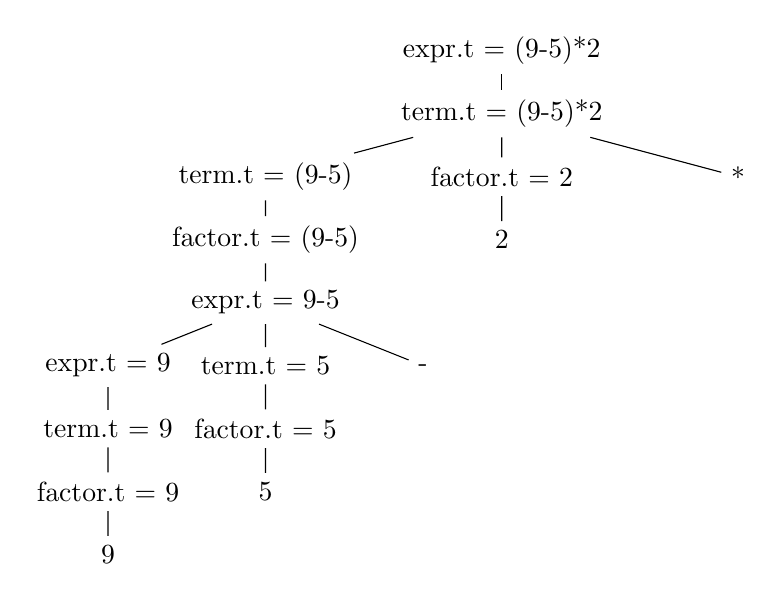
\begin{tikzpicture}[level 1/.style={level distance=8mm, sibling distance=30mm},
                    level 3/.style={level distance=8mm, sibling distance=20mm}]
  \node {expr.t = (9-5)*2}
    child { node {term.t = (9-5)*2}
      child { node {term.t = (9-5)}
        child { node {factor.t = (9-5)}
          child { node {expr.t = 9-5}
            child { node {expr.t = 9}
              child { node {term.t = 9}
                child { node {factor.t = 9}
                  child { node {9} }
                }
              }
            }
            child { node {term.t = 5}
              child { node {factor.t = 5}
                child { node {5} }
              }
            }
            child { node {-} }
          }
        }
      }
      child { node {factor.t = 2}
        child { node {2} }
      }
      child { node {*} }
    }
  ;
\end{tikzpicture}
\end{document}
